\documentclass[14pt]{extarticle}
\usepackage{extsizes}
\usepackage{geometry}
\geometry{margin=0.5in}

%% for images
\usepackage{graphicx}
\graphicspath{ {images/} }

%% language support
\usepackage[T1,T2A]{fontenc}
\usepackage[utf8]{inputenc}
\usepackage[english,russian]{babel}

\usepackage{amsmath}
\usepackage{tikz}

%% hyperrefs
\usepackage{hyperref}
\hypersetup{
    colorlinks,
    citecolor=black,
    filecolor=black,
    linkcolor=black,
    urlcolor=black
}

\title{БДЗАААААААААААААААААААААААААААААА}
\author{Ну я}

\begin{document}
\maketitle
Это нужно знать всем детям! \\\\
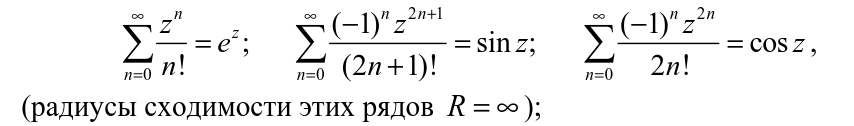
\includegraphics[width=450pt]{img1.png} \\
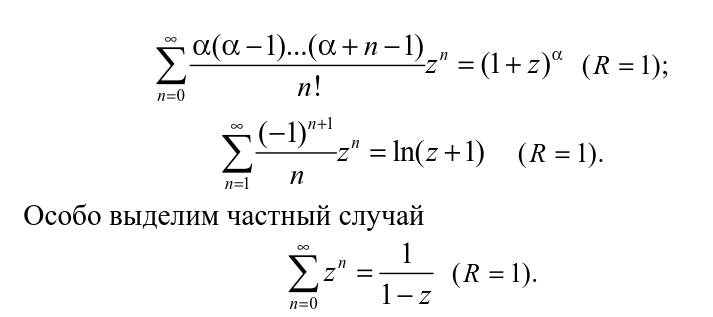
\includegraphics[width=350pt]{img2.png} \\
Удобное обозначение: \\
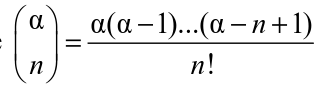
\includegraphics[width=150pt]{img3.png} \\

7. Заданную функцию $f(z)$ разложить в ряд Тейлора в точке $z_0$: 
$$f(z) = \frac{2z}{\sqrt{4-z^2}}, \ z_0 = 0$$
$$\frac{2z}{\sqrt{4-z^2}} = \frac{z}{\sqrt{1-\frac{z^2}{4}}}=
z \ * \ \left(1-\frac{z^2}{4}\right)^{-\frac{1}{2}}=
\sum_{n=0}^{\infty}\begin{pmatrix}
    -\frac{1}{2} \\
    n
\end{pmatrix}\frac{(-z^2)}{4^n}^n=$$
$$=
\sum_{n=0}^{\infty}\begin{pmatrix}
    -\frac{1}{2} \\
    n
\end{pmatrix}\frac{(-1)^n z^{2n}}{2^{2n}}$$

8. Заданную функцию $f(z)$ разложить в ряд Лорана в кольце
$a < |z-z_0| < b$ и в окрестности точки $z=\infty$:
$$f(z)=\frac{2z}{(z-1)(z^2+9)}, \ 1<|z|<3, \ z=\infty$$
$$f(z)=\frac{2z}{(z-1)(z^2+9)}=\frac{1}{5} \ \frac{1}{z-1}+
\left(-\frac{1}{5}z+\frac{9}{5}\right) \ \frac{1}{(z-3i)(z+3i)}
= f_1(z)+f_2(z)$$ \\
1) в кольце \\\\
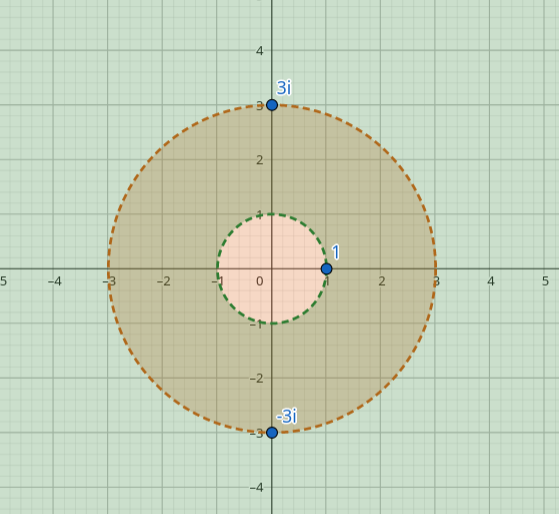
\includegraphics[width=300pt]{img4.png} \\
Точки $\pm 3i$ лежат вне кольца, потому 2е слагаемое соответствует
правильной части (раскладываем по степеням $(z-1)$); 
аналогично, точка $1$ лежит внутри кольца и 
1е слагаемое соответствует главной части (по степеням $\frac{1}{z-1}$). 

$$f_2(z) = \left(-\frac{1}{5}z+\frac{9}{5}\right) \ \frac{1}{z^2+9}=
-\frac{1}{5} \ \frac{z-9}{z^2+9}=-\frac{1}{5} 
\left(\frac{1+3i}{2} \ \frac{1}{z+3i} 
+ \frac{1-3i}{2} \ \frac{1}{z-3i}\right)=$$
$$= -\frac{1}{5} 
\left(\frac{1+3i}{2} \ \frac{1}{z - 1 + (1+3i)} 
+ \frac{1-3i}{2} \ \frac{1}{z - 1 + (1-3i)}\right)=$$
$$= -\frac{1}{5} 
\left(\frac{1}{2} \ \frac{1}{1+\frac{z - 1}{1+3i}} 
+ \frac{1}{2} \ \frac{1}{1-\frac{z-1}{1-3i}}\right)=$$
$$= -\frac{1}{10}\left(\sum_{n=0}^{\infty}(-1)^n
\frac{(z-1)^n}{(1+3i)^n}+\sum_{n=0}^{\infty}
\frac{(z-1)^n}{(1-3i)^n}\right)=$$
$$= -\frac{1}{10}\sum_{n=0}^{\infty}(z-1)^n\left(
\frac{(-1)^n}{(1+3i)^n}+\frac{1}{(1-3i)^n}\right)$$
Получим\\
$$f(z) = f_1(z) + f_2(z) = 
\left(-\frac{1}{10}\right)\sum_{n=0}^{\infty}(z-1)^n\left(
\frac{(-1)^n}{(1+3i)^n}+\frac{1}{(1-3i)^n}\right) 
+ \frac{1}{5} \ \frac{1}{z-1}$$
\end{document}
